
%!subsection{Cultural Significance of Facades and Ornament}
%!\label{subsec: FacadeandOrnament}

%!==========================
%Delve deeper into how facades reflect cultural values, societal norms, and historical contexts. Explore how different societies and civilizations have expressed their identity through architectural ornamentation and symbolism.
%!==========================
We have established a foundation for the notion that contemporary architecture is gravitating towards a renaissance of complexity.
This resurgence is catalyzed by the utilization of technology and sophisticated software analyses, enabling the creation of innovative ornamentation that seamlessly integrates functionality with cultural heritage.
This evolution paves the way for the elaboration of intricate patterns that serve as a powerful medium to express the distinct identity of the local environment, thereby rejuvenating the urban landscape.

Transitioning into the focal point of this research, we delve into the trajectory of architectural complexity within the specific realm of facades.

Facades, a paramount architectural element, have held an enduring significance for centuries due to their role as the initial point of contact with a building, acting as a boundary between the interior and the exterior, working as an interface between the living spaces and the external climate, influencing comfort and energy efficiency\cite{Kamal2020} thereby acting as the primary medium through which the structure interacts with its surroundings (Figure\ref{fig:FacadeBaroqueVsContemporary}).

%% Figure of baroque facade vs contemporary facade
     \begin{figure}[htb]
          \centering
          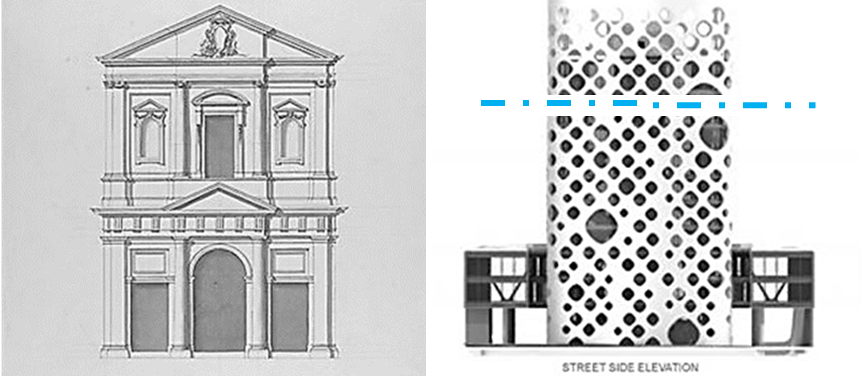
\includegraphics[width= \linewidth]{Images/BaroqueVsContemporaryfacade}
          \caption{Evolution of facade design.
          Baroque Facade 1639 by Bernini (left) vs Contemporary facade, building O-14 by Reiser + Umemoto, 21st Century (right) (\textit{Images edited from source)}}
          \label{fig:FacadeBaroqueVsContemporary}
        \end{figure}

However, much like the broader scope of architecture, the role of ornamentation and facades has also undergone evolution and transformation throughout history.
To elucidate how various societies and civilizations have conveyed their identity through architectural ornamentation and symbolism, we embark on an exploration of the interpretations given to facades by some of the most influential architects and artists of their respective eras.

%%Facade according to vitruvius

Vitruvius, a celebrated Roman architect and military engineer, in 1st century BCE, author of ``De Architectura'', a series of ten books considered as the first treatise in architecture theory\cite{Kruft1994}.
Within this work, Vitruvius advocates for three essential attributes that a building should embody: ``firmitas'' (structural soundness), ``utilitas'' (functionality), and ``venustas'' (beauty or aesthetics)\cite{Ostwald2023}.

Vitruvius places emphasis primarily on Reason, and secondarily on proportions.
It's worth highlighting that the cultural atmosphere in ancient Rome during the late first century B.C favoured the understanding of the world as a well-structured and ordered whole\cite{Lefas2000}.

Facades partake of this reasoning and in accordance to Vitruvius should not only be visually appealing but should also reflect the underlying structural integrity of the building and fulfill its intended purpose effectively(Figure\ref{fig:Vitruvianarchitecture}).
In terms of ornamentation, Vitruvius seeks to approach this subjective realm, dominated by taste, with objectivity.
He rationalizes that a pleasing appearance emerges from the harmony and balance among the components that constitute a composition\cite{Lefas2000}.

%% Figure of vitruvian Architecture
    \begin{figure}[htb]
        \centering
        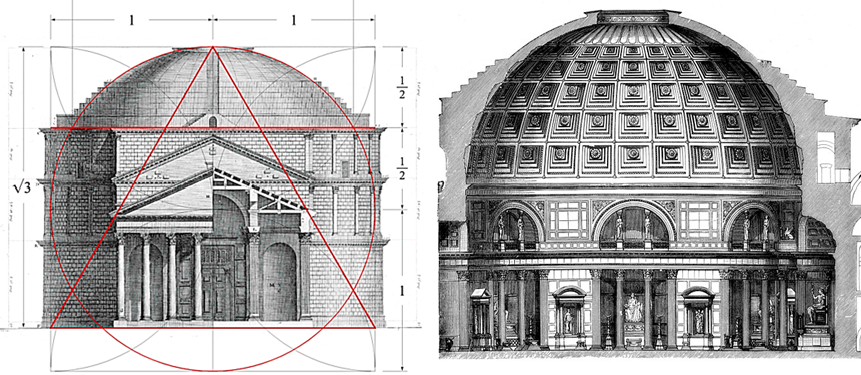
\includegraphics[width= \linewidth]{Images/VitruvianArchitecture}
        \caption{Facade and ornament according to Vitruvius, with emphasis in order symmetry and harmony. Pantheon's facade (left) and cross section(right) symmetry analysis (\textit{Images edited from source)}}
        \label{fig:Vitruvianarchitecture}
    \end{figure}

Additionally, Vitruvius determines that the deciding factor for those components would follow the principle of ``Decor'',  the  fifth  principle on his system of values that elevates simple  building  practice  into  architecture, defined as the property that  deals  with  the  «appropriate»  articulation and construction of the work on principles respecting religion, nature and social conventions\cite{Lefas2000}.

In essence, according to Vitruvius, facades and their ornamentation stem from a sense of order and rationality.
They are achieved through a harmonious equilibrium of well-considered elements that adhere to established principles, while taking into account both tradition and nature.
This approach aims to achieve beauty while also effectively fulfilling the intended purpose of the facade.

Vitruvius's contributions would have a lasting impact on the field of construction spanning centuries.
However, his work remained largely dormant for a considerable period until its revival during the Renaissance, which encompassed the 14th to the 17th century.

This resurgence continued during the Neoclassical style of the 18th century and the Ecole des Beaux-Arts style of the 19th and early 20th centuries.
This series of revivals and reinterpretations led to the rekindling of Classical architecture in the years that followed\cite{Wikipedia2023}(Figure\ref{fig:ClassicismNeoClassicism}).

%% Figure of Classicism and Neo classicism facade
     \begin{figure}[htb]
          \centering
          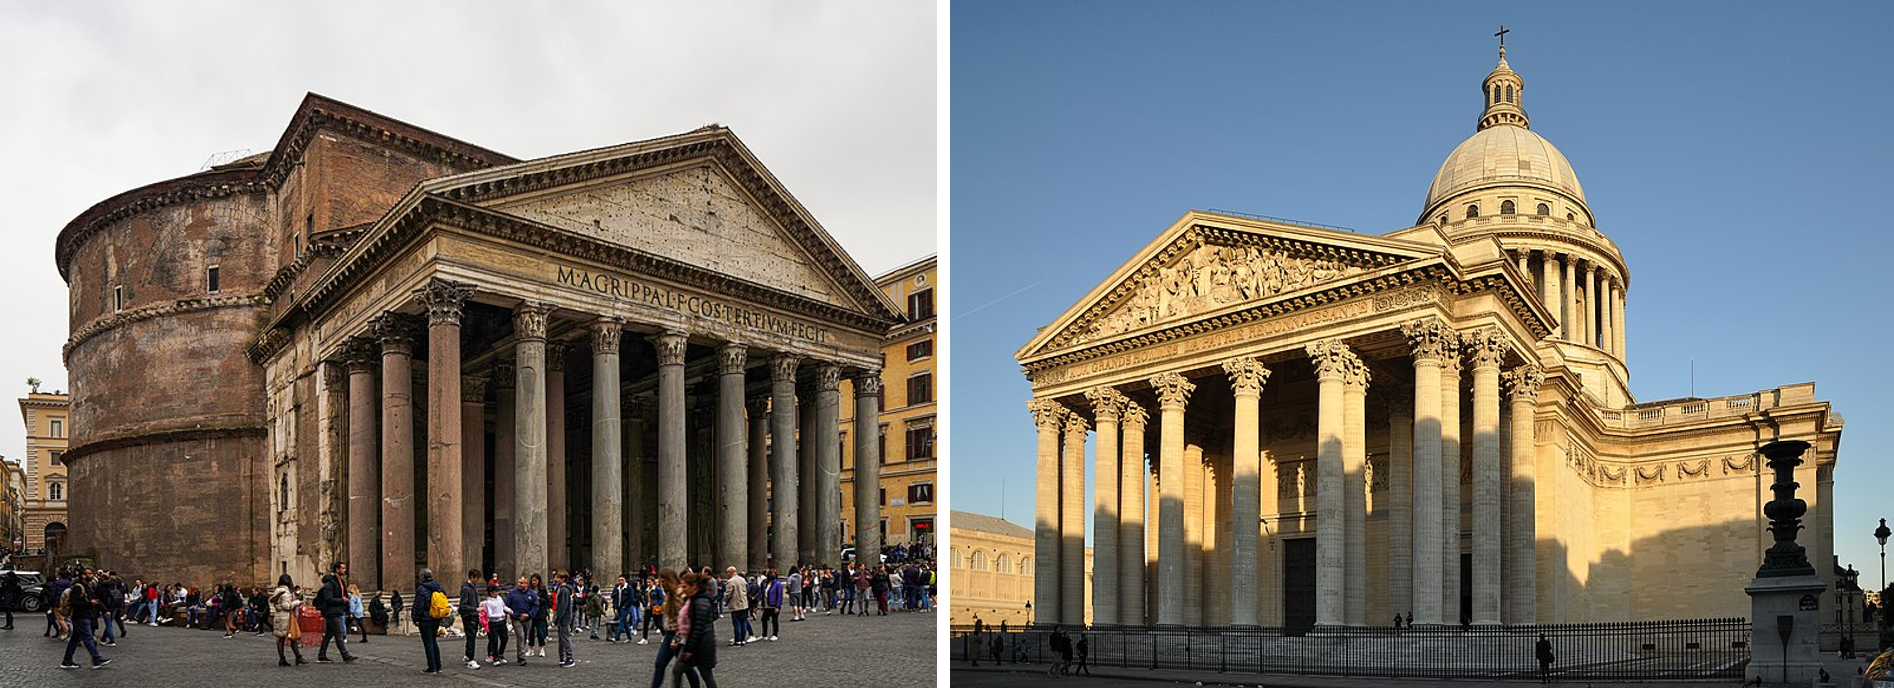
\includegraphics[width= \linewidth]{Images/ClassicismNeoClassicism}
          \caption{Continuity of Vitruvius' Influence: Classicism and Neoclassicism in Facades and Ornamentation. Architectural aesthetics rooted in order and rationality. (Left) Pantheon in Rome, constructed in 27 BC. (Right) Pantheon in Paris, erected between 1758 and 1790, Neoclassical Approach in the Mid-18th Century. (\textit{Images edited from source)}}
          \label{fig:ClassicismNeoClassicism}
        \end{figure}

%%facade according to bernini and borromini
Moving beyond the Renaissance era and into the Baroque style, a significant shift in the perception of facades and ornamentation occurs.
Francesco Borromini, a prominent Italian architect of the Baroque period, emerges as a key figure in this context.

In his exploration of facades, Borromini emphasized the dynamic relationship between a building's interior and its facade, as a form of movement of matter beyond the body, precisely because the generation of form is internal to the object itself\cite{Benjamin2006}, therefore the facade should serve as a visual representation of the internal spaces and functions of the building.

Borromini's approach to facades went beyond mere decorative elements.
He saw the facade as an opportunity to express the inner workings and spatial organization of the building.
This concept is reflected in his designs, where facades often featured intricate geometric patterns, curved forms, and sculptural elements that hinted at the internal arrangements of rooms and structures(Figure\ref{fig:BorrominiArchitecture}).

%% Figure of Baroque facade Borromini
     \begin{figure}[htb]
          \centering
          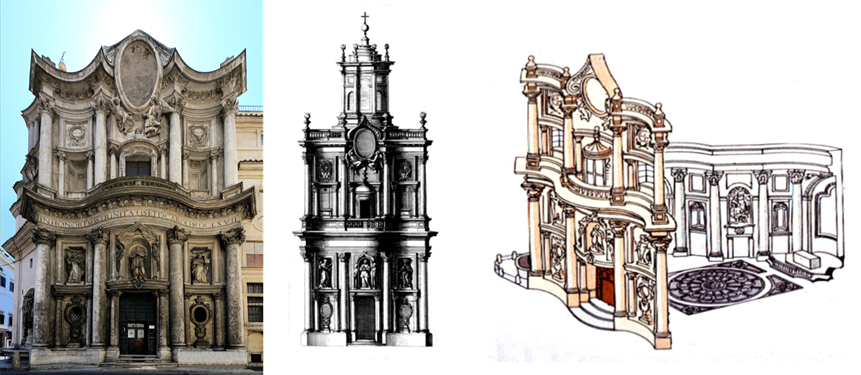
\includegraphics[width= \linewidth]{Images/BaroquefacadeBorromini}
          \caption{Borromini's Interpretation of Facade and Ornament: Elaborate geometric patterns, curved forms, and sculptural elements reflecting internal spatial arrangements. Analysis of San Carlo alle Quattro Fontane Church Facade (left) and Cross Section (right) from its construction in the 1630s, Rome. (\textit{Images edited from source)}}
          \label{fig:BorrominiArchitecture}
        \end{figure}

``Exteriors which expressively display interiorities;
interiors which fold from within and, [\ldots] which appear to invite an exterior reading while presenting an interiorized text''\cite{Biglieri2004}.
In essence, Borromini's perspective on facades went beyond surface aesthetics;
he considered them as integral components of the architectural composition that could convey deeper meanings about the building's design and purpose.

%! context on neo classic, art nouveau and art deco

Exploring the historical evolution of facades and ornamentation necessitates acknowledging distinct periods that have significantly contributed to the advancement of architectural practice.

In the trajectory from Baroque to the transformative epoch of Modernism, various architectural styles emerged, yet none attained the global influence and profound impact comparable to the preceding Classicism, which drew inspiration from the ideals of Vitruvius, and subsequently Modernism on the 20th century would bring.

For the purpose of this research, before delving into the profound shifts of Modernism, it's crucial to acknowledge certain periods that contributed to architectural understanding without causing radical shifts.

Chronologically, the evolution from Baroque to Modernism included styles like Rococo, Neoclassical, Romanticism, Gothic Revival, Victorian, Arts and Crafts, Art Nouveau, and Art Deco, each leaving their mark on architectural expression.

Notably, Neo-Classicism, Art Nouveau, and Art Deco stand out as particularly influential periods.

The Neo-Classical style of the late 18th to early 19th centuries, with a resurgence through the École des Beaux-Arts in Paris during the late 19th to early 20th centuries, reflected facades and ornamentation rooted in Vitruvian Principles and Palladian Architecture.
It emphasized formal elegance, symmetry, and grandeur, often featuring facades with balanced proportions flanked by columns (Figure\ref{fig:ClassicismNeoClassicism}).

The Art Nouveau style of the late 19th to early 20th centuries, prominent in Europe, introduced ornamentation and facades with an organic character.
This style, exemplified by figures like Gaudi, drew inspiration from nature's forms and flow lines.
Gaudi's work, for instance, used flowing,  wavy,  and  naturally  curvilinear lines that mirrored natural shapes, and mosaic-like tiles mimicking textures and colors of the natural world\cite{Nasir2022} (Figure\ref{fig:ArtNouveaustyle}).

%% Figure of Art Nouveau style  facade
     \begin{figure}[htb]
          \centering
          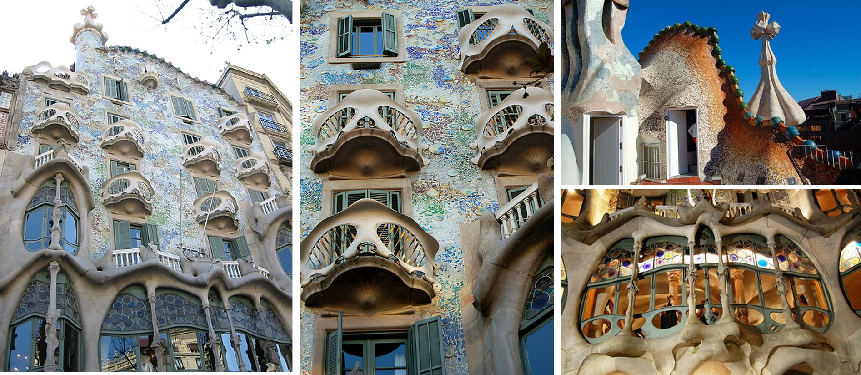
\includegraphics[width= \linewidth]{Images/ArtnouveauGaudi}
          \caption{Facade and ornament according to Art Nouveau style inspired in organic forms, illustrated by Casa Batlló in Barcelona, 1904, designed by Antoni Gaudi. (Left) Casa Batlló's iconic facade. (Middle) A close-up of the intricate mosaic work and balconies. (Upper Right) Ornate mosaic patterns on the roof and (Down Right) windows echoing the textures and colors of the natural world. (\textit{Images edited from source)}}
          \label{fig:ArtNouveaustyle}
        \end{figure}

While the Art Deco style prevalent in Europe and America during in the 1920s to early 1930s will come to rethink Facade and Ornament through the prisms of luxury and technological progress.

Characterized by its distinct attributes, Art Deco places an emphasis on crisp lines, striking geometric shapes often arranged symmetrically, and a vivid palette of high-contrast, intense colors.
This visual impact is further heightened by the incorporation of metallic surfaces, contributing to an overall ornamental effect that catches the eye\cite{Kotb2014}.

This style aimed to capture both modernity and historical nostalgia, resulting in a fusion of futuristic aspirations and references paying homage to the past (Figure\ref{fig:NeoclassicArtDeco}).

%% Figure of Art Deco style  facade
     \begin{figure}[htb]
          \centering
          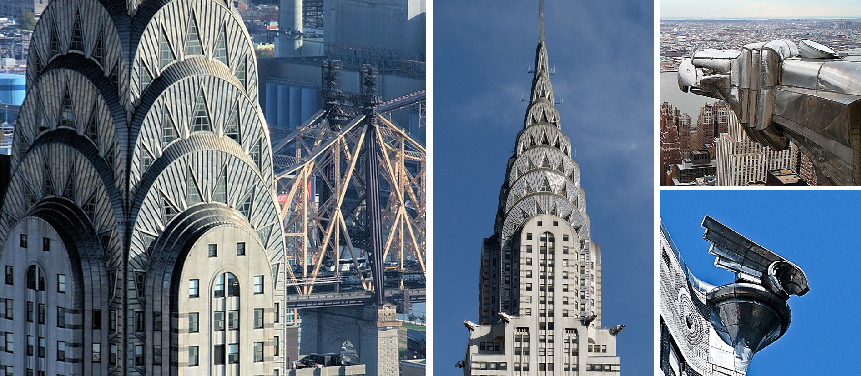
\includegraphics[width= \linewidth]{Images/ArtDecoFacade}
          \caption{Art Deco Aesthetic of the 1920s to Early 1930s:Art Deco Approach in the 1920s to Early 1930s:  Illustrated by the Chrysler Building, completed in 1930. Facade (Left) and ornamental details (Right) harmonizing futuristic aspirations with references paying homage to the past. (\textit{Images edited from source)}}
          \label{fig:NeoclassicArtDeco}
        \end{figure}

However, while these styles undoubtedly added depth and variety to architectural aesthetics, they did not bring about the same profound paradigm shifts that would later characterize the Modernist movement.

With this broader context established, the analysis will now shift its focus to the Modernist movement's transformative impact on architectural philosophy.

%! Modernism and facade according to Le Corbusier

Transitioning from the Baroque style, where facades became expressions of internal dynamics, and acknowledging the enriched insights from the Neoclassical, Art Nouveau and ArtDeco Style,  the historical evolution of facades and ornamentation takes us into the Modernist style of the 20th century—a pivotal juncture that marked one of the most significant shifts in architectural theory.

 Within this era, a radicalized interpretation of ``Form follows function'' emerged, embodying a profound departure from the conventional understanding of facades and ornamentation, partly due to a prevailing stance against ornamentation, often dismissed on moralistic grounds.

Adolf Loos' 1908 article ``Ornament and Crime'' exemplified this sentiment by advocating functional design and condemning conventional ornamentation as unnecessary\cite{Saglam2014}.

Le Corbusier, one of the most prominent figures of this epoch, and renowned for his influential work ``Towards a New Architecture'' first published in 1923, and considered by some to be the most important architectural work published in the 20th century, epitomized the spirit of the era with his distinct views on facades and ornamentation\cite{Studio2a2023}.

Embracing a minimalist and utilitarian approach, Le Corbusier believed that a facade should mirror a building's internal functions, designed in alignment with its purpose and occupants' needs.

Rooted in a human-centric design philosophy, his mantras ``Constructing the architecture of men'' and ``Men are the ones who truly matter'' underscored his commitment to prioritizing people's well-being in his designs\cite{Virseda2021}.

His manifesto ``The Five Points of a New Architecture'' further solidified his design principles.
The notion of ``Free design of the facade'' attained by separating the exterior of the building from its structural function is presented as the means through which the facade liberates itself from conventional structural limitations\cite{Corbusier1986}.

This allowed for the incorporation of large expanses of windows to provide ample natural light and ventilation, fostering a seamless connection between the interior and exterior realms.

Even during this era when ornamentation was viewed unfavorably, Le Corbusier believes in a form of functional ornamentation, as Venturi\cite{Venturi1972} would later accurately point out, Modern architecture uses expressive ornament and shuns explicit symbolic  ornament.

He would ingeniously devise methods to infuse his creations with a distinct form of ornamentation, albeit one rooted in materials' textures, structural elements, and inventive ways of articulating functionality\cite{Saglam2014} that emerged from the building's design.

For example, he used sunshades, brise-soleil, and other shading devices as a way to address climate and control light without compromising the building's aesthetic integrity.

In essence, Le Corbusier's viewpoint on facades and ornamentation epitomized clarity, rationality, and harmonious integration.
His architecture rejected superfluous adornment, and celebrated both technological advancements and structural innovation while maintaining a genuine focus on the well-being and experiences of the occupants (Figure\ref{fig:Modernistfacade}).

%% Figure of Modernist facade and ornament by Le corbusier
     \begin{figure}[htb]
          \centering
          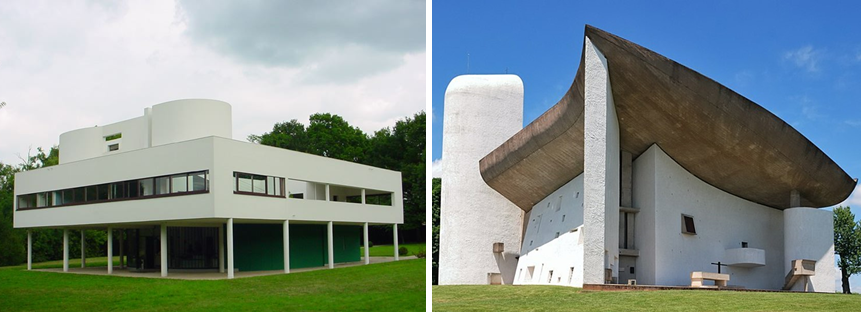
\includegraphics[width= \linewidth]{Images/ModernistFacade}
          \caption{Evolution of Functionalism: Le Corbusier's Journey towards Modernist Facade and Ornamentation. (Left) Villa Savoye, 1928--1931. (Right) Chapelle Notre-Dame-du-Haut de Ronchamp, 1955 (\textit{Images edited from source)}}
          \label{fig:Modernistfacade}
        \end{figure}

%! Postmodernism and facade according to Venturi

However, despite the innovative ideals of the Modernist movement,  it became apparent that its utopian vision didn't always materialize as intended.
While the pursuit of functionalism and simplicity was meant to create efficient and logical designs, the outcomes were not always aligned with the intended human experiences.

The Modernist approach often led to the unintentional creation of spaces that felt monotonous and detached from their cultural contexts.
The emphasis on minimalism and the rejection of ornamentation sometimes resulted in environments lacking a sense of identity and character.

The architectural pursuit of universality and timelessness would instead produce sterile, glass-cube structures\cite{Schudel2018} disregarding the importance of cultural heritage and local context, and inadvertently raise the question: Is the reinvention of form, that rejected explicit symbolism and frivolous applique ornament, inspired by the modernist ideals, yielding a Heroic and original outcome, or is it, instead, a dry expressionism, empty and boring that has distorted the whole building into one big ornament\cite{Venturi1971}.

This scrutiny of the Modernist movement's inability to adequately encompass human experiences and cultural significance, which sparked controversy during the 1960s, brings us to the influential ideas of architect and theorist Robert Venturi.

Venturi's book ``Complexity and Contradiction in Architecture'', published in 1966, marked a turning point in architectural discourse and challenged the prevailing modernist ideals.

Robert Venturi, an iconoclastic architect often hailed as the pioneer of postmodernism\cite{Schudel2018} stood firmly against the oversimplification of architecture, championing the incorporation of contradiction and complexity to yield authentic and vital creations.

The modernist ideals, heavily favoring automobile-centric urban planning, influenced the formation of cities that catered to cars rather than people.

In their thought-provoking book from 1972, ``Learning From Las Vegas'', Venturi et al.\cite{Venturi1972} put forth a compelling argument, exemplified by the stark contrast seen in places like Las Vegas, they assert that if you were to strip away the dazzling signs, what remains is not a thriving urban environment but a barren desert.

This analogy underscores the extent to which architecture had been relegated to a mere functional necessity camouflaged behind attention-grabbing signs.

Venturi et al.\cite{Venturi1972} will further explain that the oversimplification of architecture, combined with the emergence of sprawling spaces, high speeds, and intricate functions where symbols hold more significance than actual forms, has transformed architecture into symbols occupying space, rather than forming it.

This shift implies that the architectural structure itself carries minimal meaning, with the focus primarily directed towards the signs that communicate with it.

The building stands isolated from the street, often separated by vast parking lots, while the front-facing sign juts out perpendicular to the highway, detached from the building.
At the rear, the structure becomes a utilitarian afterthought, reduced to a budgetary obligation\cite{Venturi1972}.

In this scenario, the absence of signs leaves behind a vacuous atmosphere, characterized by scattered buildings that lack enclosure and cohesion.
The architecture loses its essence, mirroring a cultural void much like a desert devoid of life and enrichment.

The impact of these dynamics is not confined to the past;
instead, they continue to reverberate through the present state of our cities.
Many urban landscapes today still adhere to the principles that emerged from the modernist era.
The prioritization of cars and the resulting sprawling infrastructure persist in shaping cityscapes that often prioritize functionality over human experience.

In response to the challenges posed by the Modernist movement and its unintended consequences, Venturi would reshape the course of architectural discourse.
Notably, he will famously invert the famous dictum of Mies van der Rohe ‘Less is more’ into ‘Less is a bore'\cite{Lutolli2020}, encapsulating his bold departure from the prevailing architectural norms.

In his book ``Complexity and Contradiction in Architecture''\cite{Venturi1977}, Venturi emphasized that architecture should be responsive to the cultural context and the people who inhabit it.

His viewpoint marked a departure from the rigid modernist principles who shunned symbolism of form as an expression or reinforcement of content that dictated that architectural form was to be determined solely by program and structure, with an  occasional  assist from  intuition\cite{Venturi1972}.

Instead, he proposed a reevaluation of the role of ornament and complexity in architectural design (Figure\ref{fig:postmodernfacade}).

%% Figure of Postmodernism facade and ornament
     \begin{figure}[htb]
          \centering
          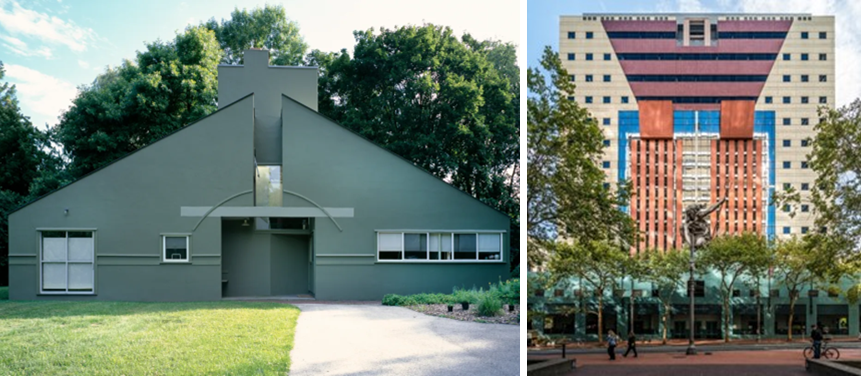
\includegraphics[width= \linewidth]{Images/PostmodernismVenturi}
          \caption{Postmodernism and the advent of complexity and contradiction (Left) Vanna Venturi House, designed by Robert Venturi and Denise Scott Brown in 1964. (Right) Portland Municipal Services Building, designed by Michael Graves, in 1982 (\textit{Images edited from source)}}
          \label{fig:postmodernfacade}
        \end{figure}

On this context, Venturi believed that a facade could communicate various meanings, evoke emotions, and respond to its cultural and contextual surroundings.

Venturi emphasized the richness of symbolism within architecture, asserting that symbols were fundamental in the architectural language, advocating for the integration of elements from historical precedents and the existing urban fabric, treating them as source materials that could be intelligently referenced or replicated to inform the design process\cite{Venturi1971}.

Importantly, Venturi's approach did not solely prioritize outward appearance;
it was deeply intertwined with the functional aspects of a building's interior, aligning with his belief that architecture should serve both utilitarian purposes and evoke meaningful experiences.

Regarding ornament, he argued that ornamentation was not inherently negative but should be used judiciously and meaningfully.

Venturi coined phrase ``Less is a bore'', suggests his approach towards ornament in what he would describe as ``the decorated shed''\cite{Venturi1972} that architecture doesn't have to be stripped of ornamentation to be considered valid.

His approach to facades, and for those that shared the postmodern movement,involved a deliberate use of various elements to add depth and complexity.
These included decorative elements like ornate moldings, intricate carvings, references to classical motifs, fragmentation of forms and the use of bright colors and patterns in the arrangement of the facade\cite{McLaughlin2023}.

Rather than adhering to a single architectural style, Venturi purposefully juxtaposed different styles, often expressed through a variety of materials and textures.
This approach aimed to create a visually stimulating experience by embracing the concept of contradiction (Figure\ref{fig:postmodernOrnamnet}).

%% Figure of Postmodernism ornament
     \begin{figure}[htb]
          \centering
          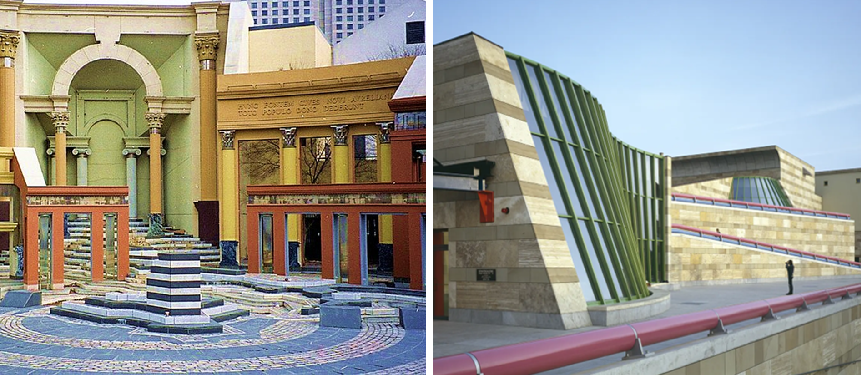
\includegraphics[width= \linewidth]{Images/PostmodernOrnament}
          \caption{Postmodernism approach to ornament using referencing different historical styles in a variety of materials and colors to create complexity. (Left) The Piazza d’Italia, New Orleans, designed by  postmodernist Charles Moore and Perez Architects, built in 1978. (Right) Neue Staatsgalerie, Stuttgart, Germany, designed by James Stirling, built in 1984 \textit{(Images edited from source)}}
          \label{fig:postmodernOrnamnet}
        \end{figure}

Furthermore, Venturi's designs exhibited a sense of playfulness.
He introduced references to historical styles, cultural symbols, and contextual connections, adding layers of meaning to his designs.

This approach to ornamentation went beyond mere decoration;
it sought to enrich the architectural experience by engaging with diverse influences and creating a dialogue with the surrounding environment.

In essence, Robert Venturi's perspective on facades and ornamentation underscored the significance of welcoming diversity, historical resonance, and meaningful expression within architectural design.

His vision urged contemporary architects to recognize a crucial reality—perfection within the architectural realm is not confined to flawless forms but also encompasses the beauty found in imperfection, across its myriad manifestations\cite{Lutolli2020}.

This eclectic and innovative approach, which drew inspiration from a renewed appreciation for historical ornamentation, boldly expanded the horizons of architectural exploration throughout the 20th century\cite{Stamp2016} paving the way for the bold explorations and boundary-pushing experiments that would characterize the late 20th century.
%! Contemporary styles start

As the 20th century progressed, architecture continued to evolve, building upon the foundations laid by modernism and postmodernism.
This era witnessed a shifting design sensibility, marked by a more dynamic and diverse approach, particularly evident in the treatment of facades and ornamentation.

We have previously stated the argument that the history of architecture, and the essence of architecture evolution, consists of an ever-changing interplay between simplicity and complexity.

In the aftermath of Postmodernism, the realm of architecture saw a diverse array of styles emerge, each carrying forward unique interpretations of facades and ornamentation in an apparent trend towards more complex design.

As Hopkins\cite{Hopkins2020} elaborates, while modernism sought clarity and simplicity in its facades, and aimed to distill architecture to its essential fundamentals, postmodernism adopted a contrasting approach embracing complexity and ornamentation and just adding more ideas, symbols on an effort to communicate what it does.

This shift marked a transition from abstract and minimalist aesthetics to a more descriptive and communicative style.

Contemporary architecture emerged as a synthesis of these previous movements.
In the realm of ornamentation, contemporary architects found a middle ground, recognizing the potential of ornament to convey meaning, context, and identity.

Ornamentation in contemporary architecture often took on a more purposeful role, serving as a bridge between tradition and innovation.

The ornamentation became a language through which buildings could communicate their cultural relevance, while also responding to the demands of a rapidly changing world.

Influenced by the advent of computer-aided design and advancements in technology, as well as driven by a sustainability agenda emphasizing efficient resource utilization, the architectural world of the late 20th century and the current 21st century has witnessed the emergence of several prominent architectural styles.

While this era lacks a unified movement, the different styles have collectively left an indelible mark on the field of architecture.

These styles include Deconstructivism, Neofuturism, High-tech modernism, Parametricism, and Pragmatic utopianism, each offering a unique perspective on architecture and design (Figure\ref{fig:contemporarytimeline}).

%% Figure of Contemporary timeline
     \begin{figure*}[htb]
          \centering
          \includegraphics[width= \linewidth]{Images/contemporaryTimeline}
          \caption{Contemporary architecture. An era of exploration. (from left to right) Desconstructivism, Neofuturism, High-tech modernism, Parametricism, Pragmatic utopinaism.  (\textit{Images edited from source)}}
          \label{fig:contemporarytimeline}
        \end{figure*}

%! Deconstructivism

In the realm of Deconstructivism, which gained prominence in the 1980s\cite{Clement2017}, architects like Frank Gehry pioneered a distinct interpretation of ornamentation taking on an unconventional and dynamic character (see Figure\ref{fig:contemporarytimeline} \textit{a}).

Deconstructivism facades challenge traditional notions, introducing the concepts of fragmentation, and fracture with non-rectilinear shapes which serve to distort and dislocate conventional building elements in a deliberate and provocative manner.

Ornamentation in this context is not applied in the traditional sense but is rather an intrinsic part of the building, such as structure and envelope and an interest in handling ideas of a structure’s surface or skin\cite{Clement2017}.
The Guggenheim museum in Bilbao, built in 1997, is a primary example of this approach towards architecture.

%! Neofuturism

Transitioning from the realm of Deconstructivism, let's now explore Neofuturism, a design movement that gained prominence in the late 20th and early 21st centuries and continues to exert influence in contemporary architecture.
This style finds a compelling embodiment in the work of Santiago Calatrava\cite{Omale2016}.

His architectural creations, exemplified by iconic structures like the Milwaukee Art Museum (refer to Figure\ref{fig:contemporarytimeline} \textit{b}), constructed in 2001, defy conventional perceptions of facades with their dynamic, seemingly in-motion forms\cite{Tyc2018}.

Neofuturism's approach to facades and ornamentation is deeply rooted in a futuristic and avant-garde aesthetic, celebrating the transformative potential of technology and the beauty of technical achievements as an art form\cite{Tyc2018}.

In contrast to the radical functionalism of modernism, Neofuturism embraces a more comprehensive functionalism.
It recognizes a multitude of functionality aspects within architectural design, including structural, pragmatic, symbolic, and social functions, as integral components of the creative process.
Moreover, Neofuturism extends its considerations to encompass environmental, urban, ethical, and aesthetic factors, all of which contribute significantly to shaping the architectural expression\cite{Omale2016}.

Characterized by sleek lines, innovative materials, and an unwavering focus on technology and functionality, Neofuturist facades lean towards minimalism.
These facades often employ steel, glass, and concrete materials, emphasizing geometric forms as key design elements\ref{fig:neofuturism}.

%% Figure of neofuturism
     \begin{figure}[htb]
          \centering
          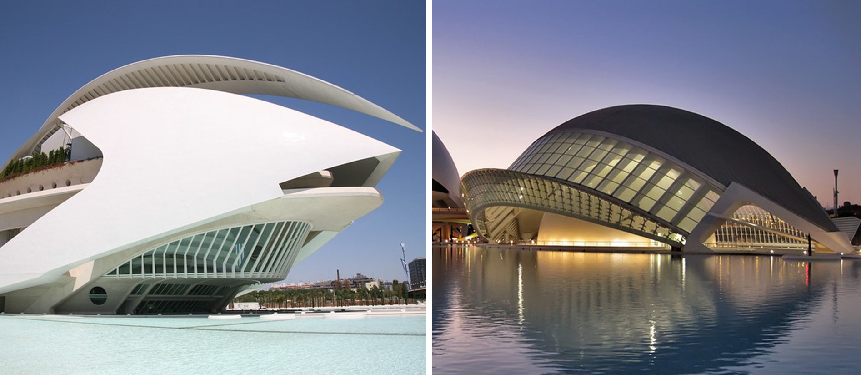
\includegraphics[width= \linewidth]{Images/neofuturism}
          \caption{Neofuturism approach to facades and ornament. (Left) Queen Sofia Palace of Arts, Valencia, Spain, designed by Santiago Calatrava , built in 2005. (Right) The City of Arts and Sciences, designed by Santiago Calatrava, built in 1996. \textit{(Images edited from source)}}
          \label{fig:neofuturism}
        \end{figure}

Neofuturist ornamentation tends to be seamlessly integrated into the building's structure and materials, prioritizing simplicity and clean lines.
The movement seeks to convey a powerful sense of progress, innovation, and a visionary perspective of the future through its architectural designs.

%! High tech modernism

Building upon the theme of technological integration, another prominent architectural style that emerged during the late 20th century, known as high-tech modernism or structural expressionism extends the exploration of facades and ornamentation in a distinctly different direction.

While neofuturism expresses its futuristic vision through dynamic forms and sleek materials, often resulting in monumental structures reminiscent of a futuristic science fiction movie, high-tech modernism takes a more measured approach.

This architectural style explores the aesthetic and functional potentials of advanced technology with a sense of refinement and restraint(refer to Figure\ref{fig:contemporarytimeline} \textit{c}).

High-tech modernism is characterized by its emphasis on technological innovation, transparency, and structural expression.
Renzo Piano and Norman Foster are influential architects associated with the high-tech modernist movement\cite{Tyc2018}.

Iconic works like The Shard (designed by Renzo Piano) and the Gherkin building (designed by Foster + Partners), both located in London, exemplify the essence of high-tech style (Figure\ref{fig:hightechmodernism}).

%% Figure of hightech modernism
     \begin{figure}[htb]
          \centering
          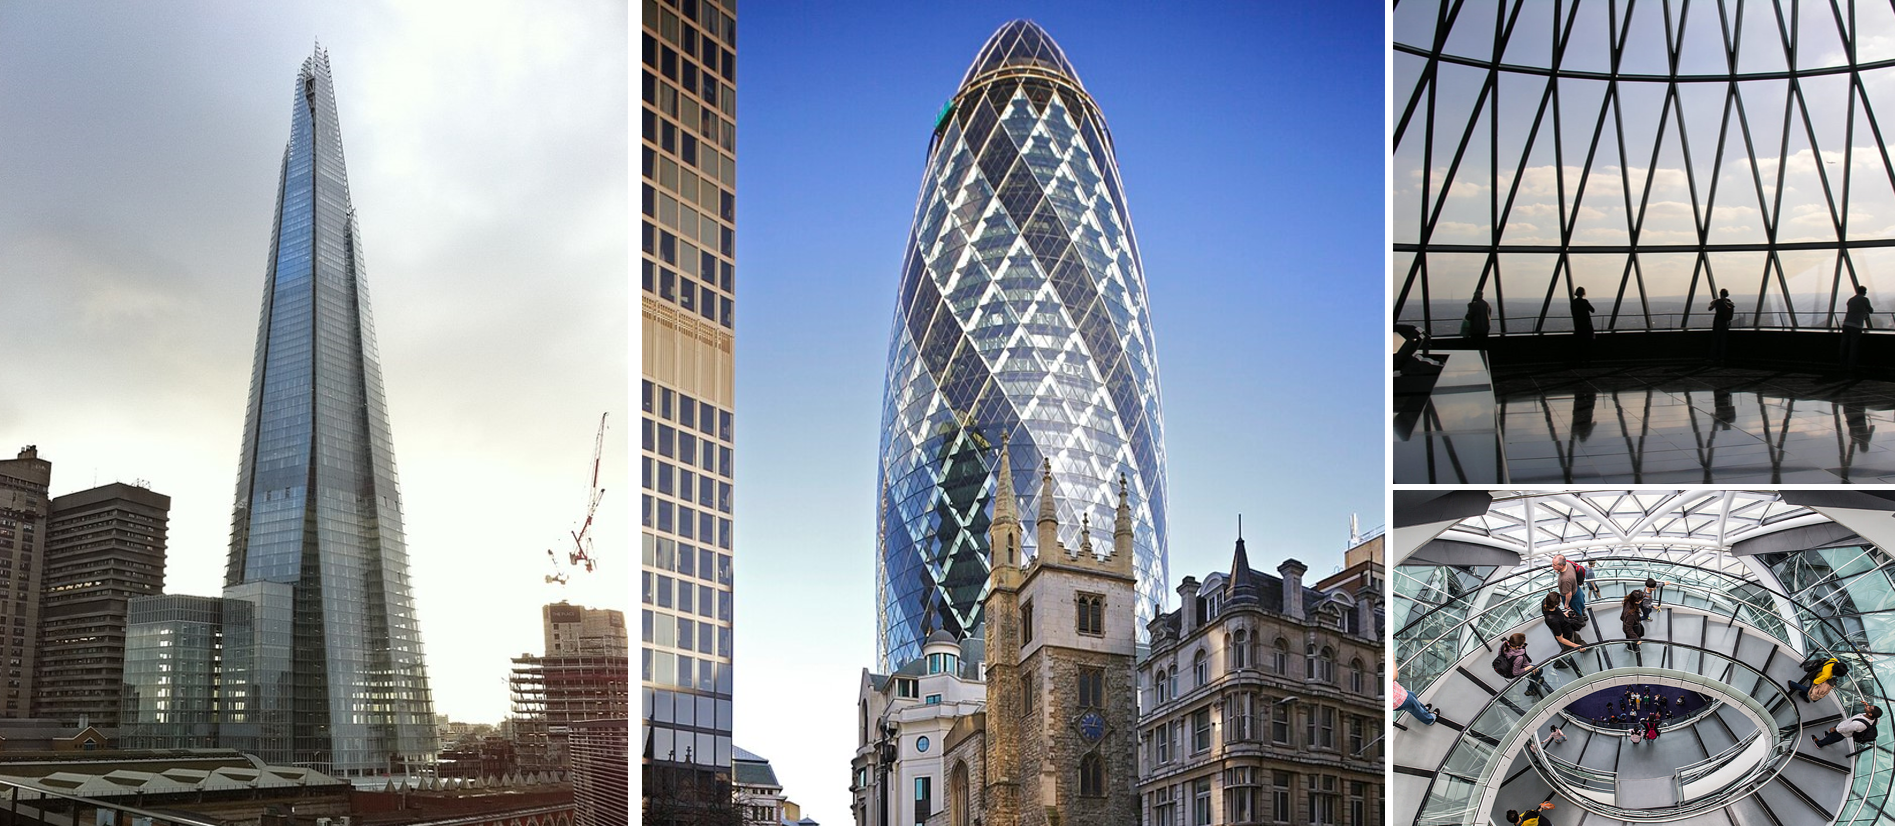
\includegraphics[width= \linewidth]{Images/hightechmodernism}
          \caption{High-tech Modernism approach to facades and ornament. (Left) The Shard, London, England, designed by Renzo Piano, built in 2012. (Right) Exterior and interior views of The Gherkin building, London, England, designed by  Foster + Partners, built in 2003 \textit{(Images edited from source)}}
          \label{fig:hightechmodernism}
        \end{figure}

In terms of facades and ornamentation, high-tech modernism often features exposed structural elements, innovative use of materials like glass and steel, and a focus on showcasing the building's inner workings.

This approach aligns seamlessly with the ethos of high-tech architects, who hold technological advancement in high regard as a driving force for architectural innovation and expression, as emphasized by Davies\cite{Davies1988}.

The aim is to showcase the building's technological components and express its functionality while maintaining a sleek and minimalist appearance.
High-tech modernism prioritizes functionality and efficiency while celebrating the aesthetic possibilities of modern technology and machines.

Le Corbusier coined the phrase ``house as a machine for living in,'' yet his own architectural creations, while inspired by this idea, remained technologically rudimentary and lacked the appearance of machines.

In contrast, High Tech buildings distinctly embody the machine aesthetic, they do look like machines.
This is not just a metaphor but a tangible source of both technology and visual inspiration\cite{Davies1988}.

It's a departure from traditional ornamentation, favoring a more industrial and minimalist aesthetic that emphasizes the beauty of engineering and technology itself.

%! Parametricism

In contrast to the emphasis on technological innovation and transparency seen in high-tech modernism, parametricism, another architectural style emerging in the late 20th century and evolving into the 21st century, takes a distinctive approach.
Often associated with renowned architects like Zaha Hadid, parametricism represents a response to technological advances, particularly in computational design (Figure\ref{fig:contemporarytimeline} \textit{d}).

Parametricism explores the integration of computational design and intricate geometries to create structures that challenge conventional ideas of facades and ornamentation.
Central to this style is the concept that all architectural elements and complexes can be shaped and adjusted through parametric means, a principle articulated by Schumacher\cite{Schumacher2010}.

Within the realm of parametricism, facades undergo a remarkable transformation, becoming dynamic and adaptive to environmental and contextual factors.
The rigid lines of traditional architecture give way to sinuous curves and intricate patterns, characterizing its formal repertoire that departs from monotonous repetition and rigid functional stereotypes\cite{Schumacher2008}.

Zaha Hadid's iconic designs, such as the Heydar Aliyev Center in Baku and the Guangzhou Opera House, exemplify this transformative approach to architecture (Figure\ref{fig:Parametricism}).

%% Figure of parametricism
     \begin{figure}[t]
          \centering
          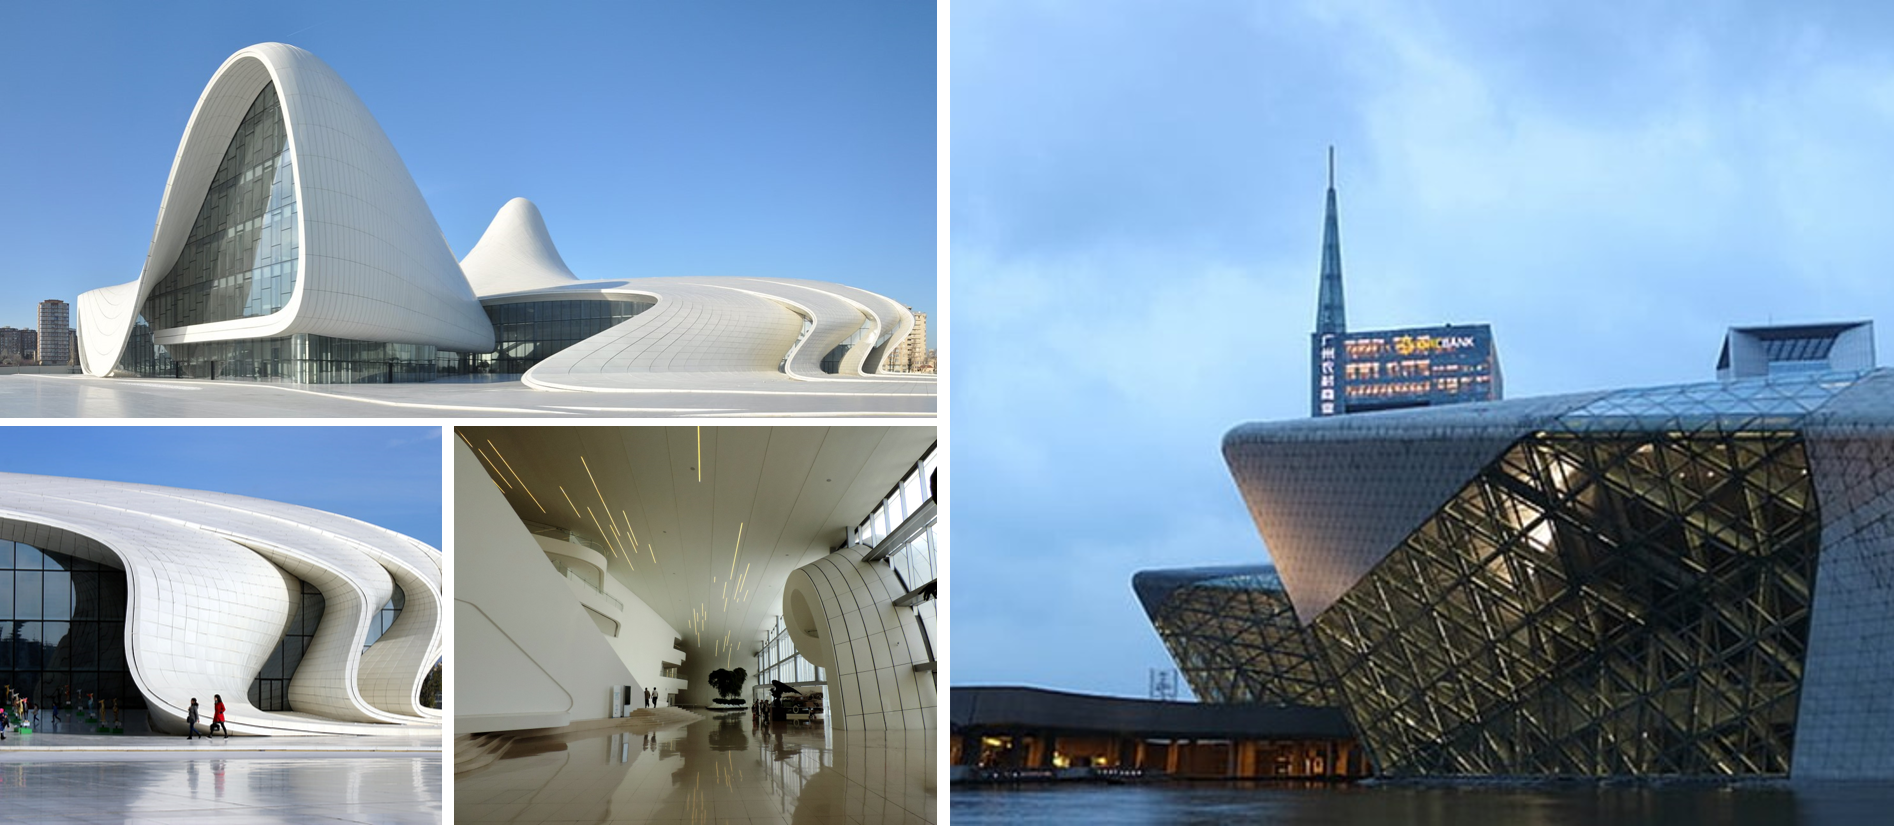
\includegraphics[width= \linewidth]{Images/Parametricism}
          \caption{Parametricism approach to facades and ornament. (Left) Exterior and interior views of Heydar Aliyev Cultural Center, Baku, Azerbaijan, designed by Zaha Hadid, built in 2012. (Right) Guangzhou Opera House,  China, designed by Zaha Hadid, built in 2010. \textit{(Images edited from source)}}
          \label{fig:Parametricism}
        \end{figure}

Parametricism leverages advanced computational tools to generate intricate and complex designs.
In this architectural style, ornamentation often emerges algorithmically, with patterns and details that respond to specific parameters or input data.
Through scripting, parametricism aims to differentiate and correlate all elements and subsystems of a design\cite{Schumacher2010}.

These parametric ornaments are highly detailed and unique to each project, enhancing the building's identity while maintaining visual continuity with the overall design.

To encapsulate, parametricism, as embodied by architects like Zaha Hadid,  stands as a transformative force in architectural design.
Through the mastery of computational tools, it harnesses the power to create intricate and dynamic structures with emphasizes in the algorithmic generation of ornamentation, resulting in highly detailed and unique designs that encapsulate the spirit of innovation and complexity, pushing the boundaries of what architecture can achieve in the 21st century.

%! Pragmatic utopianism

Transitioning from parametricism to pragmatic utopianism, we encounter yet another intriguing architectural style that emerged in response to the evolving landscape of technology, sustainability, and design philosophy.

While parametricism delves into intricate computational design and complex geometries, pragmatic utopianism embarks on a distinctive journey, combining functionality, sustainability, and a utopian vision for architecture and urban spaces.

Pragmatic utopianism, is a concept denoting the fusion of an unrealistic ideal with a practical approach, resulting in an almost perfect representation of the world.
Initially introduced by architect and bioregional planner Davidya Kasperzyk\cite{Stouhi2022}, is an architectural style that seeks to achieve an ideal world through designs that are grounded in reality (Figure\ref{fig:contemporarytimeline} \textit{e}).

Bjarke Ingels and his firm, BIG, often embody this philosophy, as Ingels himself describes it as turning pure fiction into hard fact and surreal dreams into inhabitable space\cite{Ingels2015}.
From the perspective of pragmatic utopianism, architecture should address pressing societal and environmental issues while also pushing the boundaries of innovation and aesthetics.

Ingels' projects often feature sustainable elements seamlessly integrated into the design, addressing critical environmental concerns.
For instance, the Amager Bakke plant combines waste management with a functional ski slope, ingeniously transforming a potential environmental problem into a recreational asset for the community.
This project vividly exemplifies their commitment to the idea of interweaving public infrastructure with meaningful social programs\cite{Ingels2015} (Figure\ref{fig:Pragmaticutopianism}).

%% Figure of pragmatic utopianism
     \begin{figure}[t]
          \centering
          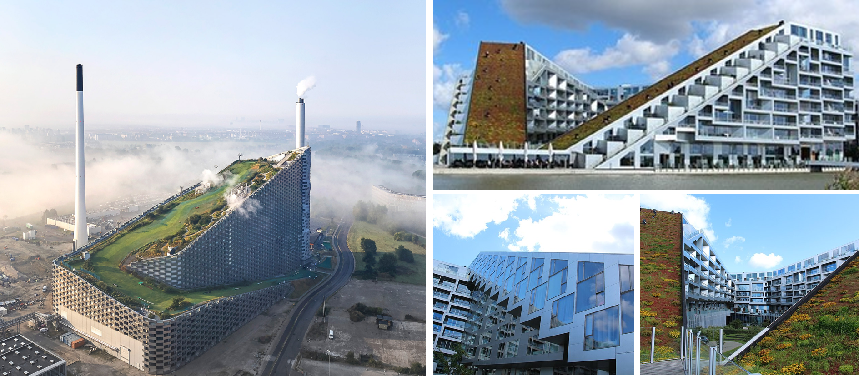
\includegraphics[width= \linewidth]{Images/pragmaticutopianism}
          \caption{Pragmatic utopianism approach to facades and ornament. (Left) Amager Bakke, a waste-to-energy power station, Copenhagen, Denmark, design by BIG, built in 2019. (Right) 8 House, Copenhagen, Denmark, design by BIG, built in 2010. \textit{(Images edited from source)}}
          \label{fig:Pragmaticutopianism}
        \end{figure}


This pragmatic utopian view emphasizes the role of architecture as a catalyst for positive change, both functionally and aesthetically, aiming to create a better future while responding to present needs .

In terms of facades and ornamentation, pragmatic utopianism takes a minimalist yet purposeful approach.
Facades are seen as not just aesthetic coverings but as functional interfaces, often a result of environmental analysis and parametric design that tailor the building envelopes to respond to different climate conditions\cite{Ingels2015}, having a crucial role in contributing positively to the environment and designed to be cost-effective and feasible, ensuring that the utopian vision is attainable within the constraints of the present.

Ornamentation within the realm of pragmatic utopianism is inherently purpose-driven, rooted in functionality, sustainability, and a desire to convey the building's mission and its positive impact on society.
It finds inspiration in the abstract art world and the imaginative realms of fictional films, where form and function harmoniously coexist\cite{Stouhi2022}.

It embodies a subtle yet essential role, seamlessly integrated into the building's form.
For instance, the graceful curves of the facade not only serve an aesthetic purpose but also communicate harmony with the nearby roadways.

Green walls and vertical gardens are incorporated not just for their visual appeal but also for their substantial contributions to improved air quality and insulation.
The facades often feature elements that cleverly serve dual functions, such as energy-efficient shading devices that simultaneously enhance the building's aesthetics.

In summary, pragmatic utopianism, as seen through the works of Bjarke Ingels, embraces a holistic approach to architecture, combining ambitious visions with practical solutions, sustainability versed in environmental analysis, and meaningful ornamentation, that culminates in designs shaped by the forces that surround them, all while addressing the pressing challenges of our time.

=============================
%edit the summary paragraph for pragmatic utopianism and add a conclusion that regards the advent of complexity

“pragmatic utopia”, a utopia that combines an unattainable ideal with pragmatism, creating an almost ideal fragment of the world.
First coined by architect and bioregional planner Davidya Kasperzyk, the term was further explored by Bjarke Ingles Group (BIG), describing an architectural style that pursues a perfect world through designs tempered by reality.\cite{Stouhi2022}

turn surreal dreams into inhabitable space, to turn fiction into fact.\cite{Ingels2015}


harness massive investments and imdue them with positive social side effect ... by proactively crossbreeding public infraestructure with social programs we can propagate new urban life-forms\cite{Ingels2015}

=============================

The inability of post-modernism and deconstructivism to formulate a new viable paradigm led to the return of modernism in the guise of minimalism as the only consistent, ideologically stringent style that confronts parametricism today.\cite{Schumacher2010}


Parametricism is the great new style after modernism.
Postmodernism and Deconstructivism have been transitional episodes that ushered in this new, long wave of research and innovation \cite{Schumacher2008}.

%establish bibliography references to defend the high tech section

% Continue writing the definition for the other styles after Deconstructivism

%Prominent contemporary architects such as Frank Gehry, Zaha Hadid, Bjarke Ingels, Santiago Calatrava, Renzo Piano, Norman Foster, and Herzog & de Meuron have contributed to the ongoing evolution of architectural expression, each bringing their distinctive approaches to facades and ornamentation.

%% add the transition to contemporary by simplifying the corntarst form modernism and post modernism like the reference from hopkins.

%% maybe add the ornament postmodernism image prepared on power point

%% Fix the ornamentation and facade descriptions with more concrete examples like do they use geometric lines colors or any specifics
%% prepare the transitioning towards the desconstructivism and revoultion of the late

    %Venturi's stance championed a departure from rigid conformity and highlighted the richness that emerges from embracing the complexities of the human experience and the interconnectedness of design with its cultural, historical, and contextual underpinnings.

%% reorganize the venturi text and seprate it from the critic of modernism. Add a las vegas analyses pic or something related to the soulless architecture. revision the interpretation of facades and ornament with citations before progressing into the contemporary

%%i need to add a paralel that our cities were generated under the modernist ideals and preference of the car which lead to the reference to Las vegas and how if you remove the signs, there is no place only a desert due to the disengage of architecture now reduce to a cheap necessity hidden behind the sign. Also add a picture of the postmodern style with a reference towards facade and ornament made clear in similar fashion as the conclusions of style written before that ussually start with in essence.

%I want to make a reflection at this point, the modernist movement utopia failed and resulted in the creation of monotonous places desensatized from its culture.
%the functionalism was misinterpreted as plainliness and resulted in dehumanized elements.
%the focus on light and glass facades ignored contextual relationship where the climate unapologetically would turn this glass boxes into ovens pradoxical ignoring the maxim of human centric design.
%architecture would follow a pattern regardless of its roots and connection to its local making them virtually indistinguishable from one another in striking contrast to the richful global diversity of the past.
%the absence of ornament was misinterpreted as the lack of effort reducing architecture to mere construction.

   %%%==========================References


